\documentclass{standalone}
\usepackage{tikz}

\begin{document}
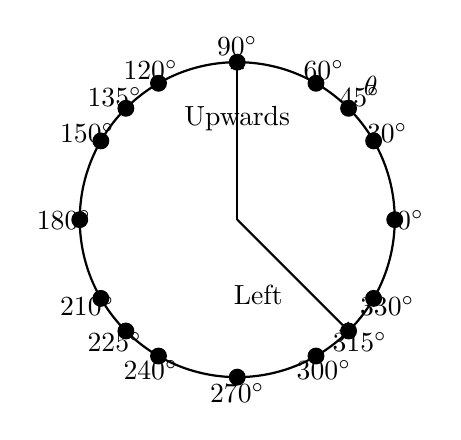
\begin{tikzpicture}[scale=2]
    % Draw the unit circle
    \draw[thick] (0,0) circle (1);
    
    % Label the points on the circle
    \foreach \angle in {0, 30, 45, 60, 90, 120, 135, 150, 180, 210, 225, 240, 270, 300, 315, 330} {
        \draw[fill=black] (\angle:1) circle (0.05);
        \node at (\angle:1.1) {$\angle^\circ$};
    }
    
    % Draw the triangle
    \coordinate (center) at (0,0);
    \coordinate (top) at (90:1);
    \coordinate (left) at (-45:1);
    \draw[thick, ->] (center) -- (top) node[midway, above] {Upwards};
    \draw[thick, ->] (center) -- (left) node[midway, below left] {Left};
    
    % Draw the angle labels for the triangle
    \node at (45:1.2) {$\theta$};
\end{tikzpicture}
\end{document}